% Capítulo 2
\chapter{Metodologia}\label{cap:metodologia}

Este estudo adota uma abordagem aplicada, com o objetivo de gerar conhecimento prático e oferecer soluções na área de avaliação educacional em programação. A pesquisa combina métodos quantitativos e qualitativos para a coleta e análise dos dados, conforme sugerido por \parencite{Gil2017},  ressalta a importância de abordagens abrangentes para investigações detalhadas orientadas para a prática. Como estratégia principal foi escolhido o estudo de caso, uma vez que esta abordagem permite explorar situações reais com limites pouco definidos, mantendo a unidade do objeto de estudo e descrevendo seu contexto. Embora tenha sido realizada uma busca sucinta por referências teóricas, essa etapa seguiu um enfoque direcionado e seletivo, com o propósito de identificar trabalhos relevantes ao tema, configurando assim uma pesquisa na literatura, porém  de escopo reduzido, com um levantamento teórico voltado à construção dos fundamentos necessário para o desenvolvimento da proposta que será discutida neste capítulo.

\section{Pesquisa de Trabalhos Relacionados}

A primeira etapa desta pesquisa consiste em explorar trabalhos recentes na literatura sobre a geração automática de questões de programação, a fim de conhecer o estado da arte e reunir a base teórica para o desenvolvimento deste estudo. Nesse processo, será realizada uma triagem com base em palavras-chave, selecionando os trabalhos por meio da análise dos títulos e resumos, seguida de uma leitura aprofundada dos trabalhos escolhidos. Essa abordagem permite identificar contribuições, desafios e lacunas relacionados à geração automática de questões de programação, fornecendo a base para responder à questão de pesquisa (\textbf{QP2}). 


\section{Desenvolvimento da Ferramenta}
Na segunda etapa, envolve a construção de um sistema capaz de executar os templates de questões de programação, gerando questões diversificadas e contextualizadas. Um mecanismo de combinação que facilita as combinações dos elementos das questões, e o uso do \gls{chatgpt} para recomendar diversos pontos de variação em cada ponto modificável do template. Após a apresentação da questão gerada e a submissão da resposta pelo aluno, o sistema, conectado à \gls{api} do \gls{chatgpt}, recebe a questão e a resposta submetida e, com base nessas informações e em um \textit{prompt} específico, gera um feedback detalhado, contribuindo para um processo de aprendizagem mais dinâmico. A Figura~\ref{fig:fluxo_desenvolvimento} apresenta um fluxograma com as principais etapas envolvidas no desenvolvimento da ferramenta, desde a definição dos requisitos até a entrega do feedback ao aluno:

\begin{figure}[ht]
	\centering
	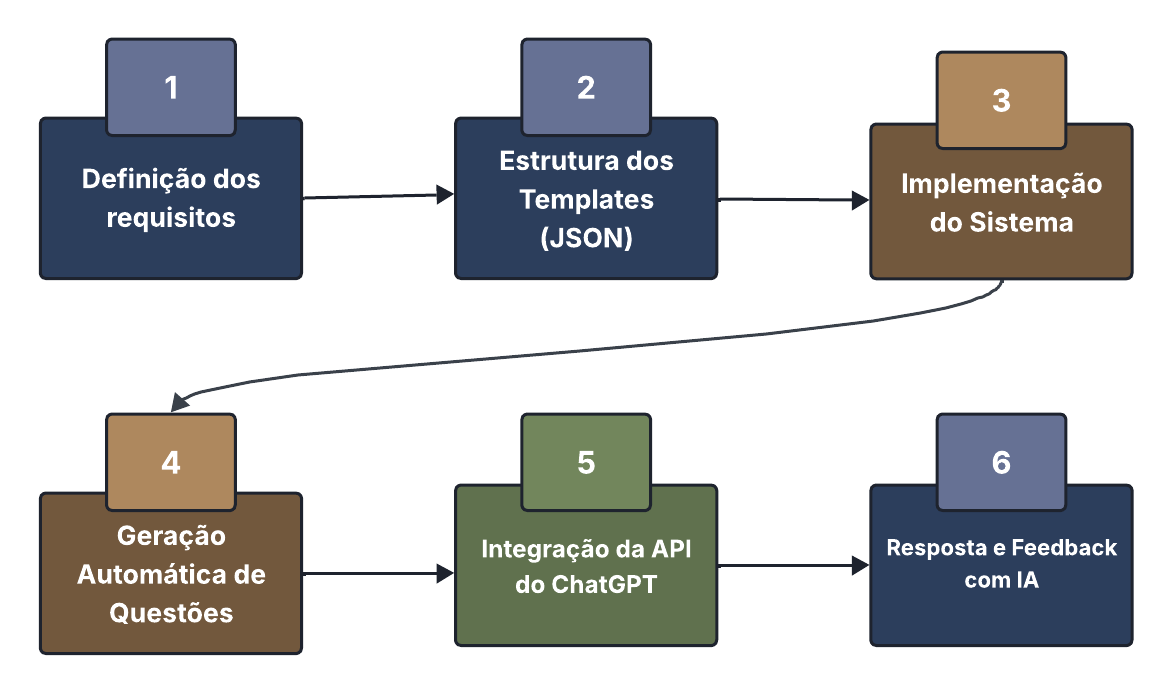
\includegraphics[width=12cm]{./imagens/capitulo2/fluxograma}
	\caption{Fluxograma : Etapas do desenvolvimento (Autoria própria, 2025)}
	\label{fig:fluxo_desenvolvimento}
\end{figure}

\subsection{Etapas do Desenvolvimento}
Com base no fluxo apresentado na figura \ref{fig:fluxo_desenvolvimento} , é possível detalhar cada uma das etapas que compõem o desenvolvimento da ferramenta. A seguir, temos os principais processos envolvidos, desde a concepção dos templates até a implementação técnica e o formato de estruturação dos dados utilizados no sistema.

\begin{enumerate}[label=\textbf{\arabic*)}]
    \item \textbf{Definição dos requisitos:} Identificação das necessidades funcionais da ferramenta, considerando os objetivos da geração automática de questões multicamadas.

    \item \textbf{Design dos templates JSON:} Criação de templates multicamadas utilizando o formato \gls{json}, escolhidos por sua leveza, eficiência e ampla aceitação em sistemas web \parencite{goyal2017, wang2011}. Esses templates estruturam elementos como enunciado, variáveis, contexto e nível de dificuldade.

    \item \textbf{Implementação do sistema:} Desenvolvimento da aplicação utilizando a linguagem Python e o framework Django. Essa escolha se justifica pela reutilização de componentes e separação clara de responsabilidades no sistema, como defendido por \parencite{rubio2017}.

    \item \textbf{Geração automática de questões:} A partir dos templates definidos, o sistema realiza combinações entre os componentes para gerar questões diversas e contextualizadas.

    \item \textbf{Integração com a API do ChatGPT:} A \gls{api} do \gls{chatgpt} é utilizada para sugerir variações nos pontos modificáveis dos templates e para processar as respostas submetidas, oferecendo feedback personalizado com base em \textit{prompts} específicos.

    \item \textbf{Resposta e feedback com IA:} Após o envio das respostas pelos estudantes, o sistema analisa as informações e retorna um feedback detalhado, promovendo um processo de aprendizagem mais interativo.
\end{enumerate}


\section{Execução do Estudo de Caso}

Nesta seção, serão apresentados os principais aspectos do estudo de caso, que busca avaliar a efetividade dos templates, coletando dados qualitativos e quantitativos para analisar desempenho, clareza e relevância das questões geradas. 


\begin{enumerate}[label=\textbf{\alph*)}]
    \item \textbf{Planejamento e Metodologia:}  
    O estudo de caso será conduzido com o objetivo de avaliar a efetividade dos templates multicamadas e do sistema de geração automática de questões. A metodologia incluirá a aplicação prática dos templates e a coleta de dados qualitativos e quantitativos para análise de desempenho, dificuldade, clareza e relevância das questões geradas. 

    \item \textbf{Participantes do Estudo:}  
    Os participantes serão professores da área de computação, que lecionam disciplinas introdutórias de programação. Eles serão responsáveis por criar templates após receber instruções específicas para estruturar o template bem como os pontos de variação nos modelos sugeridos. As questões serão geradas a partir dos templates criados, será gerada as questões cujo os temas podem ser entrada e saída, operadores lógicos, estruturas condicionais, laços de repetição e funções.

    \item \textbf{Aplicação dos Templates:}  
    Os professores participarão de atividades práticas de desenvolvimento de templates, explorando o funcionamento da ferramenta e contribuindo com a criação de novos modelos. As questões geradas pelos templates serão respondidas, permitindo aos participantes submeterem suas respostas e receberem feedback detalhado fornecido com o auxílio da Inteligência Artificial Generativa.

    \item \textbf{Coleta e Análise de Dados:}  A coleta de dados será realizada por meio da aplicação de um questionário específico que está disponível em anexo no final dessa dissertação, para avaliar a clareza e relevância das questões geradas com o intuito de identificar desafios, esforços, limitações e benefícios percebidos durante a criação e utilização dos templates. 
\end{enumerate}

\section{Resultados Esperados}

É esperado que a abordagem de geração automática de questões baseada em templates  multicamadas proporcione benefícios significativos tanto para o processo de elaboração de questões quanto para a resolução das questões. Entre esses benefícios,  um dos pontos principais é a redução do esforço necessário para criar questões tradicionais, o aumento da geração de questões em escala, elaboração de questões contextualizadas e, por fim, a melhora do engajamento dos estudantes, impulsionada pela disponibilização de feedback automatizado sobre suas respostas. Ao término do estudo de caso, será possível responder às questões de pesquisa relativas às vantagens da geração automática de questões bem como suas técnicas e modelos (\textbf{QP2}), aos desafios inerentes à criação de templates (\textbf{QP1} e \textbf{QP3}). O capítulo seguinte apresente os principais estudos relacionados destacando abordagens similares, técnicas empregas e lacunas ainda não exploradas nesta área. Sendo assim, este trabalho contribuirá para identificar limitações, oportunidades de melhorias e orientação para possíveis trabalhos futuros.

